\documentclass[tikz,border=4pt]{standalone}
% Paleta y fuentes compartidas por el libro y las figuras (única fuente de verdad).
\RequirePackage{xcolor}
\definecolor{oxido}{HTML}{B7410E}
\definecolor{cobre}{HTML}{D27D2D}
\definecolor{carbon}{HTML}{2B2B2B}
\definecolor{azul}{HTML}{1F5F8B}
\definecolor{arena}{HTML}{F4EDE4}

\usepackage{fontspec}
\setsansfont{FiraSans}[Extension=.otf,UprightFont=*-Regular,BoldFont=*-SemiBold,ItalicFont=*-Italic,BoldItalicFont=*-SemiBoldItalic]
\setmonofont{FiraMono}[Extension=.otf,UprightFont=*-Regular,BoldFont=*-Medium,Scale=0.95]
\usetikzlibrary{positioning,arrows.meta,calc,decorations.pathreplacing}
\begin{document}
\sffamily\small
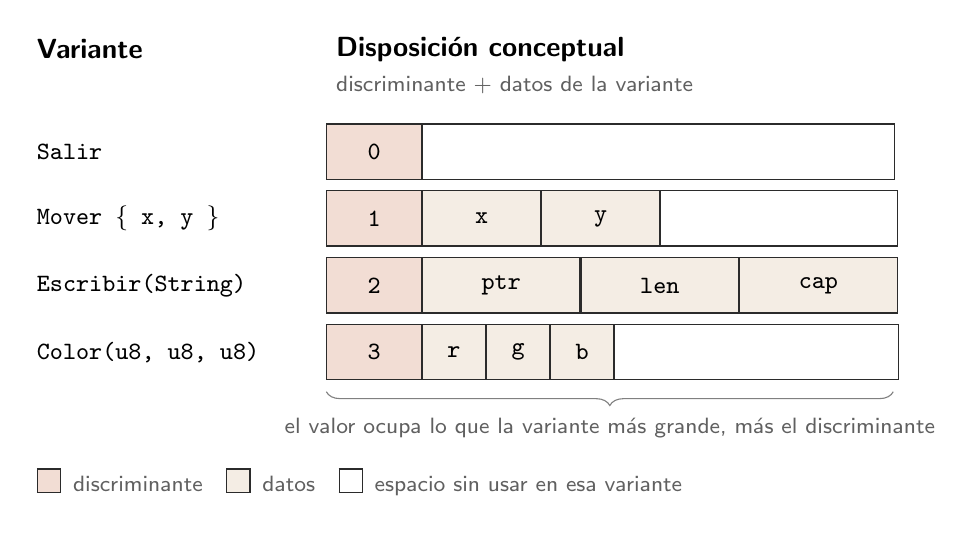
\begin{tikzpicture}[
  disc/.style={draw=carbon,fill=oxido!18,minimum height=7mm,minimum width=12mm,font=\ttfamily\small,anchor=west},
  dato/.style={draw=carbon,fill=arena,minimum height=7mm,font=\ttfamily\small,anchor=west},
  libre/.style={draw=carbon,minimum height=7mm,anchor=west,fill=white},
  nota/.style={font=\sffamily\footnotesize,text=carbon!75,anchor=west,align=left},
  >={Stealth[length=2.4mm]}]
  % Encabezados
  \node[font=\sffamily\bfseries,anchor=west] at (-0.2,0.9) {Variante};
  \node[font=\sffamily\bfseries,anchor=west] at (3.6,0.9) {Disposición conceptual};
  \node[nota] at (3.6,0.45) {discriminante + datos de la variante};
  % Filas: nombre, discriminante, datos
  \def\x{3.6}
  % Salir
  \node[font=\ttfamily\small,anchor=west] at (-0.2,-0.4) {Salir};
  \node[disc] (d0) at (\x,-0.4) {0};
  \node[libre,minimum width=60mm] at (d0.east) {};
  % Mover
  \node[font=\ttfamily\small,anchor=west] at (-0.2,-1.25) {Mover \{ x, y \}};
  \node[disc] (d1) at (\x,-1.25) {1};
  \node[dato,minimum width=15mm] (x1) at (d1.east) {x};
  \node[dato,minimum width=15mm] (y1) at (x1.east) {y};
  \node[libre,minimum width=30mm] at (y1.east) {};
  % Escribir
  \node[font=\ttfamily\small,anchor=west] at (-0.2,-2.1) {Escribir(String)};
  \node[disc] (d2) at (\x,-2.1) {2};
  \node[dato,minimum width=20mm] (a2) at (d2.east) {ptr};
  \node[dato,minimum width=20mm] (b2) at (a2.east) {len};
  \node[dato,minimum width=20mm] (c2) at (b2.east) {cap};
  % Color
  \node[font=\ttfamily\small,anchor=west] at (-0.2,-2.95) {Color(u8, u8, u8)};
  \node[disc] (d3) at (\x,-2.95) {3};
  \node[dato,minimum width=8mm] (r3) at (d3.east) {r};
  \node[dato,minimum width=8mm] (g3) at (r3.east) {g};
  \node[dato,minimum width=8mm] (b3) at (g3.east) {b};
  \node[libre,minimum width=36mm] at (b3.east) {};
  % Tamaño total
  \draw[carbon!60,decorate,decoration={brace,amplitude=5pt,mirror}]
    (\x,-3.45) -- (\x+7.2,-3.45)
    node[midway,below=6pt,nota,anchor=north] {el valor ocupa lo que la variante más grande, más el discriminante};
  % Leyenda
  \setlength{\fboxsep}{0pt}\setlength{\fboxrule}{0.4pt}
  \node[nota] at (-0.2,-4.6) {\fcolorbox{carbon}{oxido!18}{\rule{0pt}{8pt}\rule{8pt}{0pt}}\, discriminante\quad
    \fcolorbox{carbon}{arena}{\rule{0pt}{8pt}\rule{8pt}{0pt}}\, datos\quad
    \fcolorbox{carbon}{white}{\rule{0pt}{8pt}\rule{8pt}{0pt}}\, espacio sin usar en esa variante};
\end{tikzpicture}
\end{document}
